\documentclass[a4paper]{article}
\addtolength{\hoffset}{-2.25cm}
\addtolength{\textwidth}{4.5cm}
\addtolength{\voffset}{-3.25cm}
\addtolength{\textheight}{5cm}
\setlength{\parskip}{0pt}
\setlength{\parindent}{0in}

%----------------------------------------------------------------------------------------
%	PACKAGES AND OTHER DOCUMENT CONFIGURATIONS
%----------------------------------------------------------------------------------------

\usepackage{blindtext} % Package to generate dummy text
\usepackage{charter} % Use the Charter font
\usepackage[utf8]{inputenc} % Use UTF-8 encoding
\usepackage{microtype} % Slightly tweak font spacing for aesthetics
\usepackage[english]{babel} % Language hyphenation and typographical rules
\usepackage[T1]{fontenc}
\usepackage{wrapfig, subcaption, setspace}
\usepackage[font=small, labelfont=bf]{caption}
\usepackage{lastpage} % Provide ref to the last page
\usepackage{indentfirst} % Consistent indentation
\usepackage{amsfonts, amssymb, amsmath, bm} % Mathematical typesetting
\usepackage{float} % Improved interface for floating objects
\usepackage[final, colorlinks = true, 
            linkcolor = black, 
            citecolor = black]{hyperref} % For hyperlinks in the PDF
\usepackage{graphicx, multicol} % Enhanced support for graphics
\usepackage{xcolor} % Driver-independent color extensions
\usepackage{marvosym, wasysym} % More symbols
\usepackage{rotating} % Rotation tools
\usepackage{censor} % Facilities for controlling restricted text
\usepackage{listings, style/lstlisting} % Environment for non-formatted code, !uses style file!
\usepackage{pseudocode} % Environment for specifying algorithms in a natural way
\usepackage{style/avm} % Environment for f-structures, !uses style file!
\usepackage{booktabs} % Enhances quality of tables
\usepackage{tikz-qtree} % Easy tree drawing tool
\tikzset{every tree node/.style={align=center,anchor=north},
         level distance=2cm} % Configuration for q-trees
\usepackage{style/btree} % Configuration for b-trees and b+-trees, !uses style file!
\usepackage[backend=biber,style=numeric,
            sorting=nyt]{biblatex} % Complete reimplementation of bibliographic facilities
\addbibresource{ref.bib}
\usepackage{csquotes} % Context sensitive quotation facilities
\usepackage[yyyymmdd]{datetime} % Uses YEAR-MONTH-DAY format for dates
\renewcommand{\dateseparator}{-} % Sets dateseparator to '-'
\usepackage{fancyhdr} % Headers and footers
\pagestyle{fancy} % All pages have headers and footers
\fancyhead{}\renewcommand{\headrulewidth}{0pt} % Blank out the default header
\fancyfoot[L]{} % Custom footer text
\fancyfoot[C]{} % Custom footer text
\fancyfoot[R]{\thepage} % Custom footer text
\newcommand{\note}[1]{\marginpar{\scriptsize \textcolor{red}{#1}}} % Enables comments in red on margin

%----------------------------------------------------------------------------------------

\begin{document}

%-------------------------------
%	TITLE SECTION
%-------------------------------

\fancyhead[C]{}
\hrule \medskip % Upper rule
\begin{minipage}{0.295\textwidth} 
\raggedright
\footnotesize
YUCHEN WU\hfill\\   
1002060244\hfill\\
cheney.wu@mail.utoronto.ca
\end{minipage}
\begin{minipage}{0.4\textwidth} 
\centering 
\large 
Assignment 2\\ 
\normalsize 
AER1513 Fall, 2020\\ 
\end{minipage}
\begin{minipage}{0.295\textwidth} 
\raggedleft
\today\hfill\\
\end{minipage}
\medskip\hrule 
\bigskip

%-------------------------------
%	CONTENTS
%-------------------------------

\newcommand{\vect}[1]{\bm{\mathbf{#1}}}
\newcommand{\mat}[1]{\bm{\mathbf{#1}}}

\section*{Question 1} 
\textbf{TODO}\\
% As seen from Figure 2.5 in the assignment, all four sources of errors, i.e. range, bearing, translational speed and rotational speed errors, are clearly unimodal and have close-to-zero mean with a spread. Range error and translational speed error align well with the corresponding fitted Gaussian distributions. It looks like bearing error and rotational speed error have a lighter tail than the fitted Gaussian. Overall, the assumption of zero-mean Gaussian noise sounds reasonable. The standard deviation of each source of errors are given in the figure.
% \begin{eqnarray*}
%     \mat{Q}_k & = \begin{bmatrix} q^v_k & 0 \\ 0 & q^\omega_k \end{bmatrix} 
%                 = \begin{bmatrix}
%                 (0.066485)^2  & 0\\
%                 0 & (0.090477)^2 
%               \end{bmatrix} \approx
%               \begin{bmatrix}
%                 0.004420  & 0\\
%                 0 & 0.008186
%               \end{bmatrix}
%               \\
%     \mat{R}_k^l & = \begin{bmatrix} r^r_k & 0 \\ 0 & r^b_k \end{bmatrix} 
%                 = \begin{bmatrix}
%                 (0.030006)^2  & 0\\
%                 0 & (0.025912)^2
%               \end{bmatrix} \approx
%               \begin{bmatrix}
%                 0.000900 & 0\\
%                 0 & 0.000671 
%               \end{bmatrix}
% \end{eqnarray*}
% where $k = 0, ..., K$ and $l = 1, ..., L$.

% Note that in contrast to Assignment 1, we choose not to scale the noise $\mat{Q}_k$ by $T^2=0.01$ because we consider $T$ as part of the nonlinear motion model, and the noise $\vect{w}_k$ is affected by the model. We will discuss how it is affected later.

\section*{Question 2}

We combine the translation vector $\vect{r}_i^{v_k i}$ and rotation matrix $\mat{C}_{v_k i}$ into a pose matrix
\begin{equation}
\mat{T}_k = \mat{T}_{v_k i} = \begin{bmatrix}
  \mat{C}_{v_k i} & -\mat{C}_{v_k i} \vect{r}_i^{v_k i} \\ \vect{0}^T & 1
\end{bmatrix}.
\end{equation}
The state to be estimated is
\begin{equation}
    \vect{x}_{k_1: k_2} = \left\{ \vect{r}_i^{v_{k_1} i}, \mat{C}_{v_{k_1} i}, ..., \vect{r}_i^{v_{k_2} i}, \mat{C}_{v_{k_2} i} \right\} = \left\{ \mat{T}_{v_{k_1} i}, ..., \mat{T}_{v_{k_2} i} \right\}
\end{equation}
Similarly, we combine the translational velocity, $\vect{\nu}_{v_k}^{i v_k}$, and angular velocity of the vehicle, $\vect{\omega}_{v_k}^{i v_k}$, as 
\begin{equation}
    \vect{\varpi} = \begin{bmatrix}
      \vect{\nu}_{v_k}^{i v_k} \\ \vect{\omega}_{v_k}^{i v_k}
    \end{bmatrix}.
\end{equation}
The inputs from time step $k_1$ to $k_2$ can be written using the shorthand
\begin{equation}
    \vect{v} = \{ \vect{\varpi}_{k_1+1}, ..., \vect{\varpi}_{k_1+1} \}.
\end{equation}
Assume that, at time step $k$, $M_k$ landmarks are observed. The measurements can be written as
\begin{equation}
    \vect{y} = \left\{ \vect{y}^{1}_{k_1}, ..., \vect{y}^{M_{k_1}}_{k_1}, ..., \vect{y}^{1}_{k_2}, ..., \vect{y}^{M_{k_2}}_{k_2} \right\} 
\end{equation}
where $\vect{y}_k^j$ is the pixel coordinates of the point $p_j$, projected into the left and right images of the stereo camera $(u_l, v_l)$ and $(u_r, v_r)$ at time $k$, respectively.

Now we define the error terms of the inputs and measurements. For the input $\vect{\varpi}_k$, we have 
\begin{equation}
    \vect{e}_{v, k}(\vect{x}) = \ln (\underbrace{\exp(\Delta t_k \vect{\varpi}_k^\wedge)}_{\mat{\Xi}_k} \mat{T}_{k-1} \mat{T}_k^{-1})^\vee.
\end{equation}

For the measurement, $\vect{y}^j_k$, we have
\begin{equation}
    \vect{e}_{y, jk}(\vect{x}) = \vect{y}^j_k - \bar{\vect{g}}(\vect{p}_{c_k}^{p_j c_k}) = \vect{y}^j_k - \bar{\vect{g}}(\mat{D} \mat{T}_{cv} \mat{T}_{k}\vect{p}_i^{p_j, i})
\end{equation}
where $\bar{\vect{g}}$ is the nominal observation model that projects $\vect{p}_{c_k}^{p_j c_k}$ into the rectified images of an axis-aligned stereo camera, and 
\begin{eqnarray}
    \mat{D} = \begin{bmatrix}
      1 & 0 & 0 & 0 \\ 0 & 1 & 0 & 0 \\ 0 & 0 & 1 & 0 
    \end{bmatrix}, 
    \mat{T}_{cv} = \begin{bmatrix}
      \mat{C}_{cv} & -\mat{C}_{cv}\vect{\rho}_v^{cv} \\ \vect{0}^T & 1
    \end{bmatrix},
    \vect{p}_i^{p_j, i} = \begin{bmatrix}
      \rho_i^{p_j, i} \\ 1
    \end{bmatrix}
\end{eqnarray}
The weight of input and measurement errors are $\mat{Q}_k^{-1}$ and ${\mat{R}^j_k}^{-1}$, respectively, defined in Questions 1.

Finally, we define the least-squares objective function that we seek to minimize as
\begin{equation}
    J(\vect{x}_{k_1: k_2}) := \dfrac{1}{2} \vect{e}(\vect{x}_{k_1: k_2})^T \mat{T}^{-1} \vect{e}(\vect{x}_{k_1: k_2}),
\end{equation}
where we stack all the error terms and weighting matrices,
\begin{eqnarray*}
    \vect{e}(\vect{x}_{k_1:k_2}) &=& \begin{bmatrix}
      \underbrace{\vect{e}_{v, k_1+1}(\vect{x}_{k_1:k_2})\; ...\;\vect{e}_{v, k_2}(\vect{x}_{k_1:k_2})}_{\text{input errors}} \;\;
      \overbrace{\underbrace{\vect{e}_{y,1 k_1}(\vect{x}_{k_1})\;...\;\vect{e}_{y,M_{k_1} k_1}(\vect{x}_{k_1})}_{\text{measurement errors at } k_1} \;\; ... \;\; \underbrace{\vect{e}_{y,1 k_1}(\vect{x}_{k_2})\;...\;\vect{e}_{y,M_{k_2} k_2}(\vect{x}_{k_1})}_{\text{measurement errors at } k_2}}^{\text{measurement errors}}
    \end{bmatrix}\\
    \mat{T}^{-1} &=& \text{diag}(
      \mat{Q}_{k_1+1}^{-1}\; ...\; \mat{Q}_{k_2}^{-1} \;\; {\mat{R}_{k_1}^{1}}^{-1}\;...\;{\mat{R}_{k_1}^{M_{k_1}}}^{-1}\;\;...\;\;{\mat{R}_{k_2}^{1}}^{-1}\;...\;{\mat{R}_{k_2}^{M_{k_2}}}^{-1}
    )
\end{eqnarray*}


\section*{Question 3}

We first linearize the input and measurement errors at the operating point $\vect{x}_{\text{op}}$. 
Consider 
\begin{equation}
    \mat{T}_k = \exp\left( \vect{\epsilon}_k^\wedge \right).
\end{equation}
For input errors, the linearization is given by
\begin{equation}
    \vect{e}_{v, k}(\vect{x}) \approx \vect{e}_{v, k}(\vect{x}_{\text{op}}) + \underbrace{\text{Ad}\left( \mat{T}_{\text{op}, k} \mat{T}^{-1}_{\text{op}, k-1} \right)}_{\mat{F}_{k-1}} \vect{\epsilon}_{k-1} - \vect{\epsilon}_{k}
\end{equation}
where $\vect{e}_{v, k}(\vect{x}_{\text{op}}) = \ln (\mat{\Xi}_k \mat{T}_{\text{op},k-1} \mat{T}_{\text{op},k}^{-1})^\vee$ is the error evaluated at the operating point.

For measurement errors, we have that
\begin{eqnarray}
    \vect{e}_{y, jk}(\vect{x}) 
    &=& \vect{y}^j_k - \bar{\vect{g}}(\vect{p}_{c_k}^{p_j c_k})\\
    &=& \vect{y}^j_k - \bar{\vect{g}}(\mat{D} \mat{T}_{cv} \mat{T}_{k}\vect{p}_i^{p_j, i})\\
    &\approx& \vect{y}^j_k - \bar{\vect{g}}\left(\mat{D} \mat{T}_{cv}  \exp(\vect{\epsilon}_k^\wedge) \mat{T}_{\text{OP}, k}\vect{p}_i^{p_j, i}  \right)\\
    &\approx& \vect{y}^j_k - \bar{\vect{g}}\left(  \mat{D} \mat{T}_{cv}  (\vect{1} + \vect{\epsilon}_k^\wedge) \mat{T}_{\text{OP}, k}\vect{p}_i^{p_j, i}  \right)\\    
    &\approx& \vect{y}^j_k - \bar{\vect{g}}\left(  \mat{D} \mat{T}_{cv} \mat{T}_{\text{OP}, k}\vect{p}_i^{p_j, i} + \left( \mat{D} \mat{T}_{cv} (\mat{T}_{\text{OP}, k}\vect{p}_i^{p_j, i})^{\odot}  \right) \vect{\epsilon}_k \right)\\    
    &\approx& \underbrace{\vect{y}^j_k - \bar{\vect{g}}\left(  \mat{D} \mat{T}_{cv} \mat{T}_{\text{OP}, k}\vect{p}_i^{p_j, i}\right)}_{\vect{e}_{y, jk}(\vect{x}_{\text{op}})} \underbrace{- \dfrac{\partial \bar{\vect{g}}}{\partial \vect{z}}\Big|_{\vect{z}=\left(\mat{D} \mat{T}_{cv} \mat{T}_{\text{OP}, k}\vect{p}_i^{p_j, i}\right)} \left( \mat{D} \mat{T}_{cv} (\mat{T}_{\text{OP}, k}\vect{p}_i^{p_j, i})^{\odot}  \right)}_{\mat{G}_{jk}} \vect{\epsilon}_k 
\end{eqnarray}
where
\begin{eqnarray}
    \dfrac{\partial \bar{\vect{g}}}{\partial \vect{z}} = \begin{bmatrix}
      \frac{f_u}{z} & 0 & - \frac{f_u x}{z^2}\\
      0 & \frac{f_v}{z} & - \frac{f_v y}{z^2}\\
      \frac{f_u}{z} & 0 & - \frac{f_u (x-b)}{z^2}\\
      0 & \frac{f_v}{z} & - \frac{f_v y}{z^2}\\
    \end{bmatrix}
    \text{with} \quad \vect{z} = \begin{bmatrix}
      x & y & z
    \end{bmatrix}
\end{eqnarray}

Then, we define the following stacked quantities for the Gauss-Newton setup,
\begin{eqnarray}
    \delta \vect{x} &=& \begin{bmatrix}
      \vect{\epsilon}_{k_1} & \vect{\epsilon}_{k_1+1} & \dots & \vect{\epsilon}_{k_2} 
    \end{bmatrix}^T, \\
    \vect{e}(\vect{x}_{\text{op}}) &=& \begin{bmatrix}
      \vect{e}_{v,k_1}(\vect{x}_{\text{op}})\; ...\;\vect{e}_{v, k_2}(\vect{x}_{\text{op}}) \;\;
      \vect{e}_{y,1 k_1}(\vect{x}_{\text{op}})\;...\;\vect{e}_{y,M_{k_1} k_1}(\vect{x}_{\text{op}}) \;\; ... \;\; \vect{e}_{y,1 k_1}(\vect{x}_{\text{op}})\;...\;\vect{e}_{y,M_{k_2} k_2}(\vect{x}_{\text{op}})
    \end{bmatrix}^T\\
    \mat{H} &=& \begin{bmatrix}
      -\mat{F}_{k_1} & \mat{1}          & &&\\
                     & -\mat{F}_{k_1+1} & \mat{1} \\
      &&& \mat{1} & \\
      &&& \mat{F}_{k_2-1} & \mat{1}\\
      %%%%%%%%%%%%%%%%%%%%%%%%%%%%%%%%
      \mat{G}_{1,k_1}\\
      \mat{G}_{2,k_1}\\
      \vdots\\
      \mat{G}_{M_{k_1},k_1}\\
      &\mat{G}_{1,k_1+1}\\
      &\mat{G}_{2,k_1+1}\\
      &\vdots\\
      &\mat{G}_{M_{k_1+1},k_1+1}\\
      &&\ddots\\
      &&\ddots\\
      &&\ddots\\
      &&\ddots\\
      &&&\mat{G}_{1,k_2}\\
      &&&\mat{G}_{2,k_2}\\
      &&&\vdots\\
      &&&\mat{G}_{M_{k_2},k_2}
    \end{bmatrix},\\
    \mat{T} &=& \text{diag} \left(
      \mat{Q}_{k_1+1}\; ...\; \mat{Q}_{k_2} \;\; {\mat{R}_{k_1}^{1}}\;...\;{\mat{R}_{k_1}^{M_{k_1}}}\;\;...\;\;{\mat{R}_{k_2}^{1}}\;...\;{\mat{R}_{k_2}^{M_{k_2}}} \right)
\end{eqnarray}

The quadratic approximation to the objective function is then
\begin{equation}
    J(\vect{x}) \approx J(\vect{x}_{\text{op}}) - \vect{b}^T \delta \vect{x} + \dfrac{1}{2} \delta \vect{x}^T \mat{A} \delta \vect{x}
\end{equation}
where
\begin{equation}
    \mat{A} = \mat{H}^T \mat{W}^{-1}\mat{H}, \quad \vect{b} = \mat{H}^T \mat{W}^{-1} \vect{e}(\vect{x}_{\text{op}})
\end{equation}

Minimizing with respect to $\delta \vect{x}$, we have 
\begin{equation}
    \mat{A} \delta \vect{x}^* = \vect{b}
\end{equation}
for the optimal perturbation
\begin{equation}
    \delta \vect{x}^* = \begin{bmatrix}
      \vect{\epsilon}_{k_1}^* \\ \vect{\epsilon}_{k_1+1}^* \\ \ddots \\ \vect{\epsilon}_{k_2}^*
    \end{bmatrix}
\end{equation}

Finally, we update our operating point thorugh the original perturbation scheme,
\begin{equation}
    \mat{T}_{\text{op}, k} \leftarrow \exp\left( {\vect{\epsilon}_k^*}^{\wedge} \right) \mat{T}_{\text{op}, k}
\end{equation}

\section*{Question 4}

\begin{figure}[H]
    \centering
    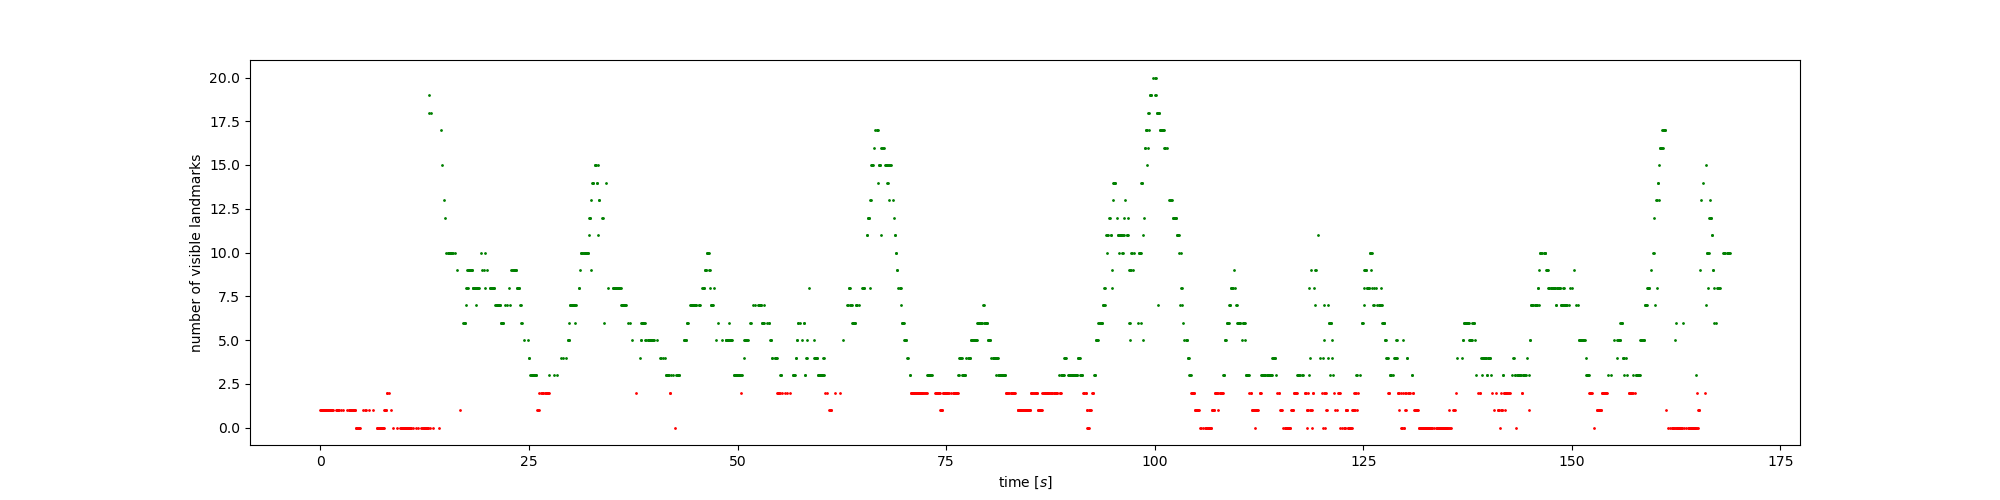
\includegraphics[width=\textwidth]{code/num_visible.png}
    \caption{Number of visible landmarks.}
    \label{fig:4}
\end{figure}

\section*{Question 5}

\begin{figure}[H]
    \centering
    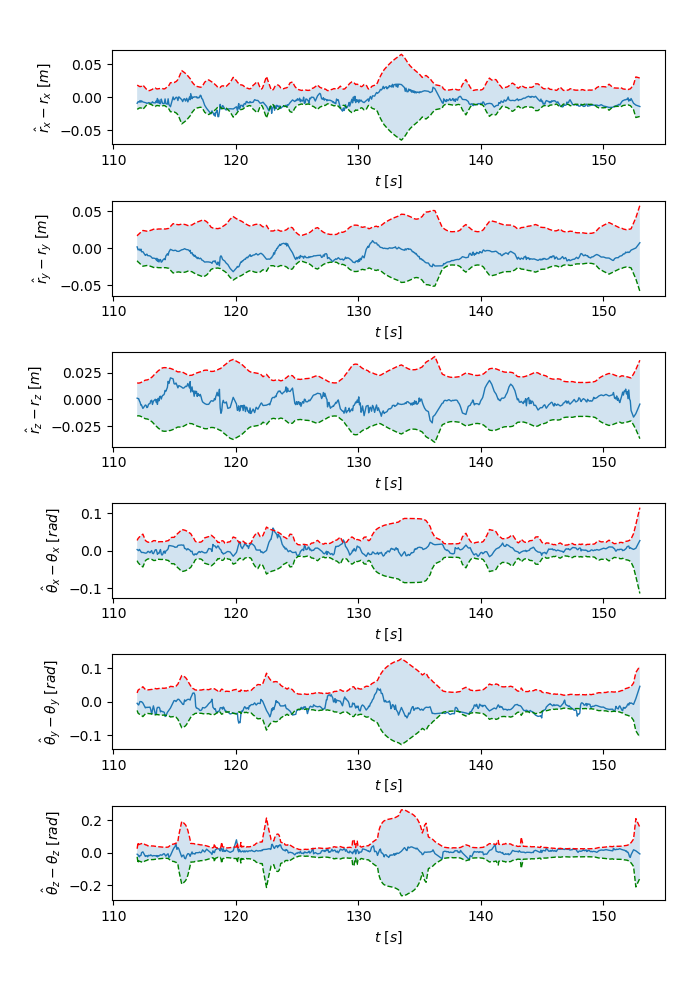
\includegraphics[width=0.9\textwidth]{code/batch.png}
    \caption{Batch.}
    \label{fig:5a}
\end{figure}

\begin{figure}[H]
    \centering
    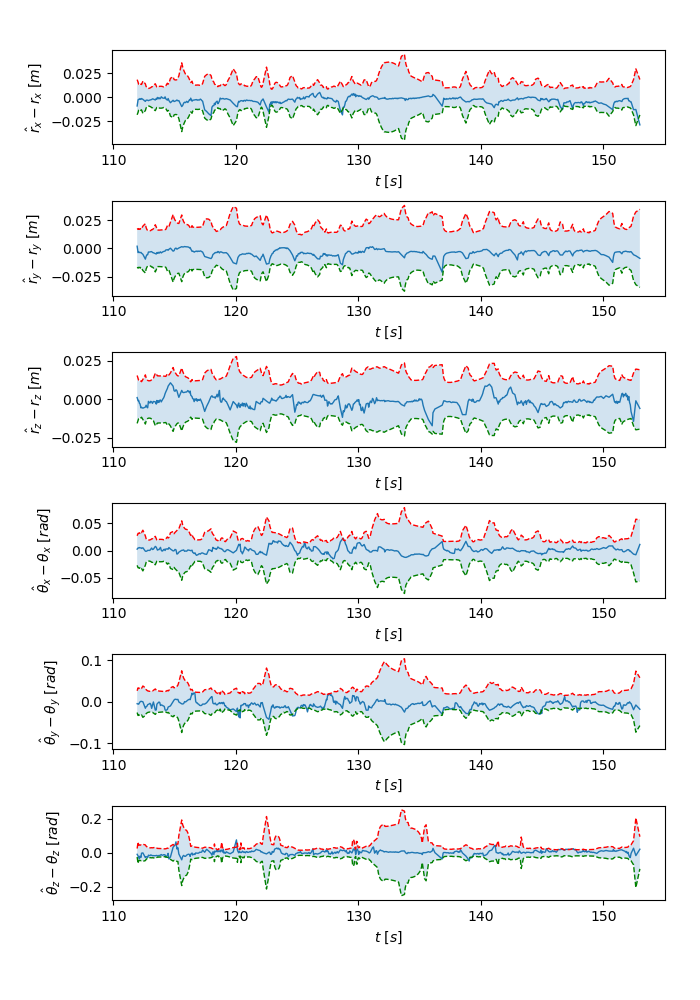
\includegraphics[width=0.9\textwidth]{code/sliding_window_50.png}
    \caption{Sliding window 50.}
    \label{fig:5b}
\end{figure}

\begin{figure}[H]
    \centering
    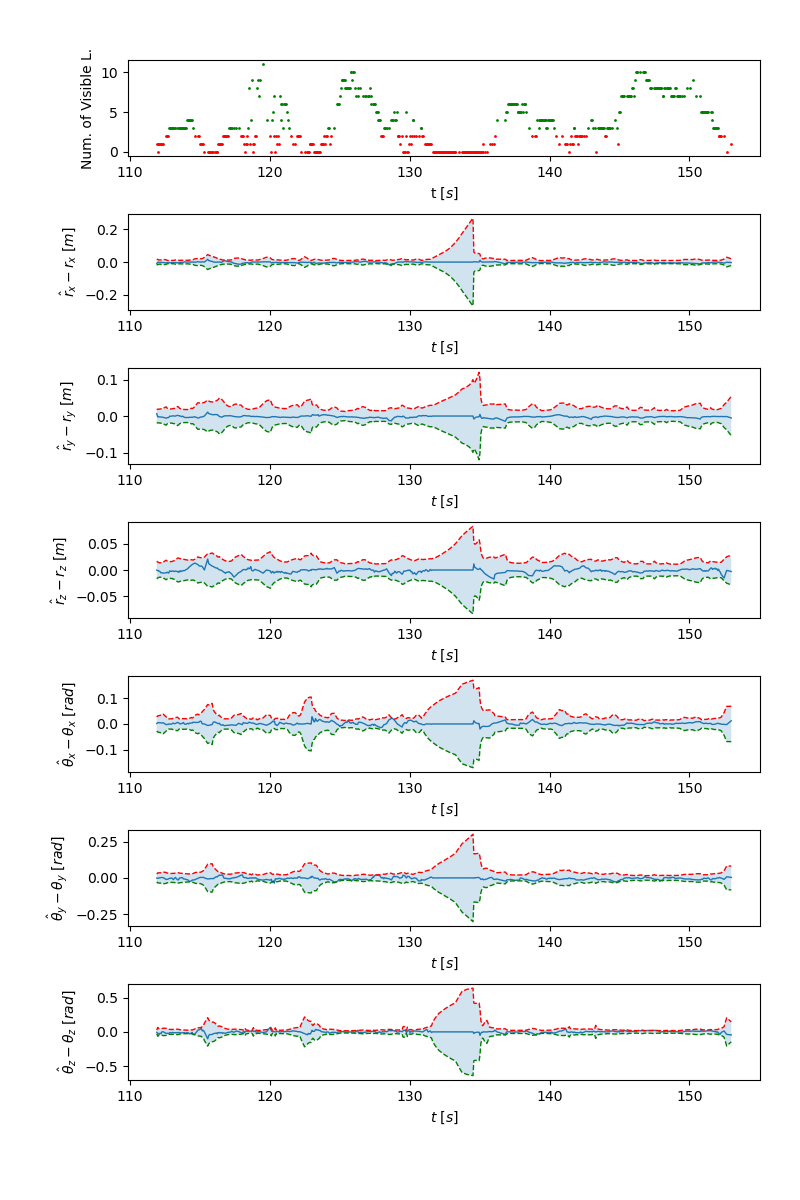
\includegraphics[width=0.9\textwidth]{code/sliding_window_10.png}
    \caption{Sliding window 10.}
    \label{fig:5c}
\end{figure}


\clearpage
\printbibliography

\appendix

\clearpage
\section{Source Code}
\label{sourcecode}

\begin{lstlisting}[language=Python, basicstyle=\small]
import os
import numpy as np
from numpy.linalg import inv
from scipy.linalg import block_diag
from scipy.io import loadmat
import matplotlib
import matplotlib.pyplot as plt
from matplotlib.animation import FuncAnimation, FFMpegWriter
from matplotlib.patches import Ellipse

# Configure matplotlib
matplotlib.use("TkAgg")
matplotlib.rcParams["pdf.fonttype"] = 42
matplotlib.rcParams["ps.fonttype"] = 42
SMALL_SIZE = 10
MEDIUM_SIZE = 12
BIGGER_SIZE = 16
plt.rc("font", size=MEDIUM_SIZE)        # controls default text sizes
plt.rc("figure", titlesize=MEDIUM_SIZE) # fontsize of the figure title
plt.rc("axes", titlesize=MEDIUM_SIZE)   # fontsize of the axes title
plt.rc("axes", labelsize=SMALL_SIZE)    # fontsize of the x and y labels
plt.rc("xtick", labelsize=SMALL_SIZE)   # fontsize of the tick labels
plt.rc("ytick", labelsize=SMALL_SIZE)   # fontsize of the tick labels
plt.rc("legend", fontsize=SMALL_SIZE)   # legend fontsize

# Helpers
wrap_to_pi = lambda th: (th + np.pi) % (2 * np.pi) - np.pi

# Load data
data = loadmat('dataset2.mat')
start_id, stop_id = 0, None
K = data["t"].shape[0]
for k, v in data.items():
  try:
    if v.shape[0] == K:
      data[k] = v[start_id:stop_id]
  except:
    pass

# Problem specific parameters
K = data["x_true"].shape[0] # number of timesteps
T = 0.1                     # sampling period
d = data["d"][0, 0]         # distance b/t robot center & laser range finder
rmax = 10                   # maximum range (will be changed later)

# Problem specific vectors and matrices (refer to Barfoot, 2017 Chapter 4.2.3)
Q = np.array([[data["v_var"][0, 0], 0.], [0., data["om_var"][0, 0]]])

Rl = np.array([[data["r_var"][0, 0], 0.], [0., data["b_var"][0, 0]]])
R = lambda l: block_diag(*[Rl for k in range(int(l.shape[0] / 2))])

f = lambda x, v: x + T * np.array([
    [np.cos(x[2, 0]), 0],
    [np.sin(x[2, 0]), 0],
    [0, 1],
]) @ v

F = lambda x, v: np.array([
    [1, 0, -T * np.sin(x[2, 0]) * v[0, 0]],
    [0, 1, T * np.cos(x[2, 0]) * v[0, 0]],
    [0, 0, 1],
])

W = lambda x: T * np.array([
    [np.cos(x[2, 0]), 0],
    [np.sin(x[2, 0]), 0],
    [0, 1],
])

dx = lambda x, l: l[0, 0] - x[0, 0] - d * np.cos(x[2, 0])
dy = lambda x, l: l[1, 0] - x[1, 0] - d * np.sin(x[2, 0])

gl = lambda x, l: np.array([
    [np.sqrt(dx(x, l)**2 + dy(x, l)**2)],
    [np.arctan2(dy(x, l), dx(x, l)) - x[2, 0]],
])
g = lambda x, l: np.concatenate(
    [gl(x, l[2 * k:2 * k + 2]) for k in range(int(l.shape[0] / 2))], axis=0)

dgldx = lambda x, l: np.array([
    [-(dx(x, l)**2 + dy(x, l)**2)**(-1 / 2) * dx(x, l)],
    [dy(x, l) / (dx(x, l)**2 + dy(x, l)**2)],
])
dgldy = lambda x, l: np.array([
    [-(dx(x, l)**2 + dy(x, l)**2)**(-1 / 2) * dy(x, l)],
    [-dx(x, l) / (dx(x, l)**2 + dy(x, l)**2)],
])
dgldth = lambda x, l: np.array([
    [(dx(x, l)**2 + dy(x, l)**2)**(-1 / 2) *
     (dx(x, l) * d * np.sin(x[2, 0]) - dy(x, l) * d * np.cos(x[2, 0]))],
    [
        -(dx(x, l) * d * np.cos(x[2, 0]) + dy(x, l) * d * np.sin(x[2, 0])) /
        (dx(x, l)**2 + dy(x, l)**2) - 1
    ],
])
Gl = lambda x, l: np.concatenate(
    (dgldx(x, l), dgldy(x, l), dgldth(x, l)), axis=1)
G = lambda x, l: np.concatenate(
    [Gl(x, l[2 * k:2 * k + 2]) for k in range(int(l.shape[0] / 2))], axis=0)

Nl = lambda _=None: np.eye(2)
N = lambda x, l: block_diag(*[Nl() for k in range(int(l.shape[0] / 2))])


def ekf(x0, P0, vs, rs, bs, lall, x_trues=np.array([])):
  global K, rmax

  x_hats = [x0]
  P_hats = [P0]

  x_hat = x0
  P_hat = P0
  for k in range(1, K):
    # terminal output
    print("EKF: step {} - {:4.2f}%".format(k, k / K * 100), end='\r')

    # control input
    v = vs[k:k + 1, :].T

    # filter observations according to rmax
    r = rs[k, :]
    b = bs[k, :]
    obs_idx = np.argwhere(np.logical_and(r > 0, r < rmax)).reshape(-1)
    has_obs = len(obs_idx) > 0
    r = r[obs_idx, None]
    b = b[obs_idx, None]
    y = np.concatenate((r, b), axis=1).reshape((-1, 1))
    l = lall[obs_idx].reshape((-1, 1))

    # predictor
    x_op = x_hat if x_trues.size == 0 else x_trues[k - 1] # x_op is at k-1
    x_op[2, 0] = wrap_to_pi(x_op[2, 0])
    x_hat[2, 0] = wrap_to_pi(x_hat[2, 0])

    P_check = F(x_op, v) @ P_hat @ F(x_op, v).T + W(x_op) @ Q @ W(x_op).T
    P_check = 0.5 * (P_check + P_check.T)

    x_check = f(x_hat, v)
    x_check[2, 0] = wrap_to_pi(x_check[2, 0])

    if has_obs:
      x_op = x_check if x_trues.size == 0 else x_trues[k]
      x_op[2, 0] = wrap_to_pi(x_op[2, 0])

      # Kalman gain
      Km = P_check @ G(x_op, l).T @ inv(
          G(x_op, l) @ P_check @ G(x_op, l).T +
          N(x_op, l) @ R(l) @ N(x_op, l).T)

      # corrector
      P_hat = (np.eye(x_op.shape[0]) - Km @ G(x_op, l)) @ P_check
      P_hat = 0.5 * (P_hat + P_hat.T)

      obs_err = y - g(x_check, l)
      obs_err[range(1, len(l), 2)] = wrap_to_pi(obs_err[range(1, len(l), 2)])
      x_hat = x_check + Km @ obs_err
    else:
      P_hat = P_check
      x_hat = x_check
    x_hat[2, 0] = wrap_to_pi(x_hat[2, 0])

    # store results
    x_hats.append(x_hat)
    P_hats.append(P_hat)

  print("EKF: step {} - 100.0% - done!".format(K))
  return np.array(x_hats), np.array(P_hats)


# true states [x, y, om]
x_trues = np.concatenate(
    (data["x_true"], data["y_true"], wrap_to_pi(data["th_true"])),
    axis=1)[..., None]
# true landmark locations
l = data["l"]
# input sequence
vs = np.concatenate((data["v"], data["om"]), axis=1)
# observations
rs = data["r"]
bs = data["b"]


def plot_q4(x, x_true, P, t, id):
  global num_figure, K

  for ts in [0, 1000]:
    if ts > K:
      continue
    num_figure += 1

    dx = (x - x_true).squeeze()
    dx[:, 2] = wrap_to_pi(dx[:, 2])
    stdx = np.array([np.sqrt(np.diag(p)) for p in P])

    fig = plt.figure(num_figure)
    fig.set_size_inches(5, 5)
    fig.subplots_adjust(left=0.16,
                        right=0.95,
                        bottom=0.1,
                        top=0.95,
                        wspace=0.6,
                        hspace=0.6)

    plt.subplot(311)
    plt.plot(t[ts:], dx[ts:, 0], linewidth=1.0)
    plt.plot(t[ts:], -3 * stdx[ts:, 0], "r--", linewidth=1.0)
    plt.plot(t[ts:], +3 * stdx[ts:, 0], "g--", linewidth=1.0)
    plt.fill_between(t[ts:], -3 * stdx[ts:, 0], 3 * stdx[ts:, 0], alpha=0.2)
    plt.xlabel(r"$t$ [$s$]")
    plt.ylabel(r"$\hat{x} - x$ [$m$]")
    if ts != 0:
      plt.ylim([-0.2, 0.2])
    print("Starting time: ", ts, " average dx: ",
          np.linalg.norm(dx[ts:, 0], ord=2)**2)

    plt.subplot(312)
    plt.plot(t[ts:], dx[ts:, 1], linewidth=1.0)
    plt.plot(t[ts:], -3 * stdx[ts:, 1], "r--", linewidth=1.0)
    plt.plot(t[ts:], +3 * stdx[ts:, 1], "g--", linewidth=1.0)
    plt.fill_between(t[ts:], -3 * stdx[ts:, 1], 3 * stdx[ts:, 1], alpha=0.2)
    plt.xlabel(r"$t$ [$s$]")
    plt.ylabel(r"$\hat{y}-y$ [$m$]")
    if ts != 0:
      plt.ylim([-0.2, 0.2])
    print("Starting time: ", ts, " average dy: ",
          np.linalg.norm(dx[ts:, 1], ord=2)**2)

    plt.subplot(313)
    plt.plot(t[ts:], dx[ts:, 2], linewidth=1.0)
    plt.plot(t[ts:], -3 * stdx[ts:, 2], "r--", linewidth=1.0)
    plt.plot(t[ts:], +3 * stdx[ts:, 2], "g--", linewidth=1.0)
    plt.fill_between(t[ts:], -3 * stdx[ts:, 2], 3 * stdx[ts:, 2], alpha=0.2)
    plt.xlabel(r"$t$ [$s$]")
    plt.ylabel(r"$\hat{\theta}-\theta$ [$rad$]")
    if ts != 0:
      plt.ylim([-0.2, 0.2])
    print("Starting time: ", ts, " average dth: ",
          np.linalg.norm(dx[ts:, 2], ord=2)**2)

    os.makedirs('figures', exist_ok=True)
    plt.savefig("figures/q4-{}-{}.png".format(id, ts))


num_figure = 0

print("Q4(a)...")
for rmax in [5, 3, 1]:
  x0_hat = np.concatenate(
      (data["x_true"][:1], data["y_true"][:1], wrap_to_pi(
          data["th_true"][:1])),
      axis=1).T
  P0_hat = np.diag((1, 1, 0.1))
  x_hats, P_hats = ekf(x0_hat, P0_hat, vs, rs, bs, l)
  plot_q4(x_hats, x_trues, P_hats, data["t"][:, 0], "a-" + str(rmax))

print("Q4(b)...")
for rmax in [5, 3, 1]:
  x0_hat = np.array([[1.], [1.], [0.1]])
  P0_hat = np.diag((1, 1, 0.1))
  x_hats, P_hats = ekf(x0_hat, P0_hat, vs, rs, bs, l)
  plot_q4(x_hats, x_trues, P_hats, data["t"][:, 0], "b-" + str(rmax))

print("Q4(b)'...") # a different initial guess
for rmax in [5, 3, 1]:
  x0_hat = np.array([[100.], [100.], [2.0]])
  P0_hat = np.diag((1, 1, 0.1))
  x_hats, P_hats = ekf(x0_hat, P0_hat, vs, rs, bs, l)
  plot_q4(x_hats, x_trues, P_hats, data["t"][:, 0], "b2-" + str(rmax))

print("Q4(c)...")
for rmax in [5, 3, 1]:
  x0_hat = np.concatenate(
      (data["x_true"][:1], data["y_true"][:1], wrap_to_pi(
          data["th_true"][:1])),
      axis=1).T
  P0_hat = np.diag((1, 1, 0.1))
  x_hats, P_hats = ekf(x0_hat, P0_hat, vs, rs, bs, l, x_trues=x_trues)
  plot_q4(x_hats, x_trues, P_hats, data["t"][:, 0], "c-" + str(rmax))

print("Q5...")
num_figure += 1

rmax = 1
x0_hat = np.concatenate(
    (data["x_true"][:1], data["y_true"][:1], wrap_to_pi(data["th_true"][:1])),
    axis=1).T
P0_hat = np.diag((1, 1, 0.1))
x_hats, P_hats = ekf(x0_hat, P0_hat, vs, rs, bs, l)

x_trues = x_trues.squeeze()
x_hats = x_hats.squeeze()

fig = plt.figure(num_figure)
ax = plt.axes(aspect=1)
plt.title(
    r"EKF estimation with $r_{max}=1$, $\hat{x}_0=x_0$ and $\hat{P}_0=$diag$\{1, 1, 0.1\}$"
)
plt.xlabel(r"$x$ [$m$]")
plt.ylabel(r"$y$ [$m$]")
plt.xlim([-2, 10])
plt.ylim([-4, 4])
plt.scatter(data["l"][:, 0], data["l"][:, 1], c="k", s=3)
x_true_p = plt.scatter([], [], c="b", s=3)
x_hat_p = plt.scatter([], [], c="r", s=3)

cov = P_hats[0, :2, :2]
lmda, v = np.linalg.eig(cov)
lmda = np.sqrt(lmda)

ell = Ellipse(xy=x_hats[0, :2],
              width=3 * lmda[0] * 2,
              height=3 * lmda[1] * 2,
              angle=np.rad2deg(np.arctan2(v[1, 0], v[0, 0])),
              fc="r",
              ec="r",
              alpha=0.2)


def init():
  x_true_p.set_offsets(x_trues[0:1, :2])
  x_hat_p.set_offsets(x_hats[0:1, :2])
  ax.add_artist(ell)
  return x_true_p, x_hat_p, ell


def animate(i, *args):
  x_true_p.set_offsets(x_trues[i:i + 1, :2])
  x_hat_p.set_offsets(x_hats[i:i + 1, :2])

  cov = P_hats[i, :2, :2]
  lmda, v = np.linalg.eig(cov)
  lmda = np.sqrt(lmda)
  ell.set_center(x_hats[i, :2])
  ell.set_width(3 * lmda[0] * 2)
  ell.set_height(3 * lmda[1] * 2)
  ell.set_angle(np.rad2deg(np.arctan2(v[1, 0], v[0, 0])))
  return x_true_p, x_hat_p, ell


anim = FuncAnimation(fig,
                     animate,
                     init_func=init,
                     frames=K,
                     interval=5,
                     blit=True)
os.makedirs('figures', exist_ok=True)
writervideo = FFMpegWriter(fps=60)
anim.save("figures/AER1513_A2.mov", writer=writervideo)

# plt.show()
print("Finished!")
\end{lstlisting}

\end{document}
